\chapter{Circular Motion, continued}
\section{Review of Circular Motion Basics}
We have previously discussed circular motion in Chapter~\ref{chap:circular_1}, so let's do a quick review of the important concepts before we move on to rotational dynamics.

We have rotational kinematics, which describes the motion of objects rotating around a fixed axis. The key variables in rotational kinematics are angular displacement ($\theta$), angular velocity ($\omega$), and angular acceleration ($\alpha$). These variables are analogous to linear displacement, velocity, and acceleration in linear kinematics.

\begin{table}[H]
\centering
\begin{tabular}{l l}
Linear motion & Rotational motion \\ \hline
$v = v_0 + a t$ & $\omega = \omega_0 + \alpha t$ \\[4pt]
$x = x_0 + v_0 t + \tfrac{1}{2} a t^2$ & $\theta = \theta_0 + \omega_0 t + \tfrac{1}{2} \alpha t^2$ \\[4pt]
$v^2 = v_0^2 + 2a(x - x_0)$ & $\omega^2 = \omega_0^2 + 2\alpha(\theta - \theta_0)$
\end{tabular}
\caption{Kinematic equations for linear and rotational motion.}
\label{tab:kinematics}
\end{table}

When an object such as a wheel or a disk rotates about an axis, each point on the object moves along a circular path centered on that axis. The total distance traveled by a point during one complete rotation is the circumference of its circular path, which is given by $ C = 2\pi r $. The rotation of the object is described by an angle $ \theta $, usually measured in radians, where one full rotation corresponds to $ 2\pi $ radians.

\section{Rigid Bodies}\index{rigid body}
Although all points on a rotating disk pass through the same angular displacement $ \theta $ in the same amount of time, they do not all travel the same distance. Points farther from the axis of rotation move along larger circles and therefore cover more distance during each rotation, even though the angular displacement is the same for all points. As a result, points farther from the axis have greater linear velocity and greater linear (tangential) acceleration than points closer to the center, as described by the relationships $ v = r\omega $ and $ a = r\alpha $. We call this points part of a \emph{rigid body}.

A rigid body is an idealized object in which the distances between all points remain constant, even when forces are applied. All points along a radial line have the same angular displacement, angular velocity, and angular acceleration.

In other words, a rigid body does not deform: it does not stretch, compress, or bend. This assumption allows the object to be treated as a single system in which all parts move in a predictable way relative to one another.

In rotational motion, treating an object as a rigid body means that:

\begin{itemize}
  \item All points in the object rotate together around a common axis.
  \item The angular velocity ($\omega$) and angular acceleration ($\alpha$) are the same for all points in the rigid body.
  \item The linear velocity ($v$) and linear acceleration ($a$) of points in the rigid body depend on their distance ($r$) from the axis of rotation, following the relationships $v = r\omega$ and $a = r\alpha $.
\end{itemize}

This idea maintains for many of the problems and concepts we will discuss in this chapter.
\section{Torque}
Let's think about pushing a box along a frictionless surface. There is a linear relationship between how hard you push and how much the box accelerates. What if, instead, you apply the same force to a merry-go-round fixed at a central pivot? Where can you push the merry-go-round for the highest rotation? Obviously you cannot push the merry-go-round linearly (as it is fixed to the ground), so how far will the merry-go-round rotate? All of these questions can be answered by the concept of \emph{torque}. 
\begin{figure}[H]
\centering
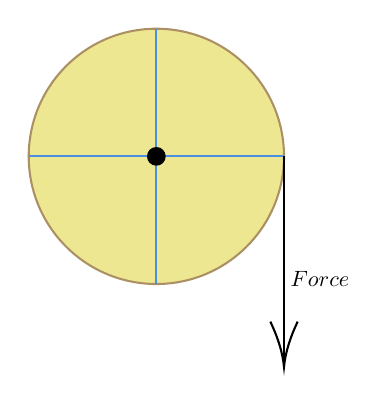
\begin{tikzpicture}[x=0.75pt,y=0.75pt,yscale=-1,xscale=1]

%Shape: Circle
\draw[color={rgb,255:red,170;green,144;blue,99},draw opacity=1,
      fill={rgb,255:red,238;green,231;blue,145},fill opacity=1]
(14,76.5) .. controls (14,42.53) and (41.53,15) .. (75.5,15)
.. controls (109.47,15) and (137,42.53) .. (137,76.5)
.. controls (137,110.47) and (109.47,138) .. (75.5,138)
.. controls (41.53,138) and (14,110.47) .. (14,76.5) -- cycle ;

%Axes/diameter lines (blue)
\draw[color={rgb,255:red,74;green,144;blue,226},draw opacity=1]
(75.5,138) -- (75.5,15) ;
\draw[color={rgb,255:red,74;green,144;blue,226},draw opacity=1]
(14,76.5) -- (137,76.5) ;

%Center point
\draw[fill={rgb,255:red,0;green,0;blue,0},fill opacity=1]
(71.5,76.5) .. controls (71.5,74.29) and (73.29,72.5) .. (75.5,72.5)
.. controls (77.71,72.5) and (79.5,74.29) .. (79.5,76.5)
.. controls (79.5,78.71) and (77.71,80.5) .. (75.5,80.5)
.. controls (73.29,80.5) and (71.5,78.71) .. (71.5,76.5) -- cycle ;


%Force arrow
\draw (137,76.5) -- (137,176) ;
\draw[shift={(137,178)}, rotate=270, color={rgb,255:red,0;green,0;blue,0}, line width=0.75]
(21.86,-6.58) .. controls (13.9,-2.79) and (6.61,-0.6) .. (0,0)
.. controls (6.61,0.6) and (13.9,2.79) .. (21.86,6.58);

%Label
\draw (139,130.65) node [anchor=north west,inner sep=0.75pt,xscale=0.8,yscale=0.8] {$Force$};

\end{tikzpicture}
\caption{Merry-go-round with a singular applied force.}
\end{figure}

\index{torque}
Torque is the concept of \emph{rotational force}. Applying a torque to a surface, a \emph{rigid body}, that has a fixed rotational pivot will cause the rigid body to \emph{accelerate} around the pivot, ultimately producing an \emph{angular acceleration}. 

Imagine pushing open a door that is bound to a hinge on one side of the door. Pushing open the door at a point close to the hinge will require large amount of Torque, while pushing closer to the door handle and farther away from the hinge is much easier to do, and requires less Torque. 

Alternatively, think of a wrench rotating a large bolt. It will require more force from your arm closer towards the pivot, while pushing at the edge of the wrench will require less force to produce an equivalent torque.

FIXME Door diagram or wrench diagram or both

\index{torques}\index{torque}
\begin{mdframed}[frametitle = {Torque}, style = important]
Torque, represented through the greek letter \tau (tau), is defined as
\begin{equation}
    \tau = rF
    \label{eq:torque_perp}
\end{equation}
where $F$ is a force perpendicular to 
\begin{equation}
    \tau = r F \sin\theta
    \label{eq:torque_sin}
\end{equation}
Notice that the torque around a pivot depends on the distance from the pivot, $r$, and the angle from the radius vector \theta. The $\sin\theta$ indicates that only the \emph{perpendicular} part of the force impacts the torque. This is equivalent to the cross product of the two vectors:
\begin{equation}
    \tau = r \times F
    \label{eq:torque_cross}
\end{equation}
Torque has units of $\text{Newton-meters}$, but in this case, it is not an energy form, so cannot be equated to $\text{Joules}$. Torque is an \emph{vector}, not a scalar.
\end{mdframed}

Let's do an example proving this.

\textbf{Question}: A rod with a fixed end is being pulled by a tension force of $50 \,\text{N}$ at a $40^\circ$ angle from the horizontal, at a distance of $2 \,\text{m}$. Find the Torque on the rod.

% Diagram made with Mathcha
\tikzset{every picture/.style={line width=0.75pt}} % default line width


\begin{figure}[H]
\centering
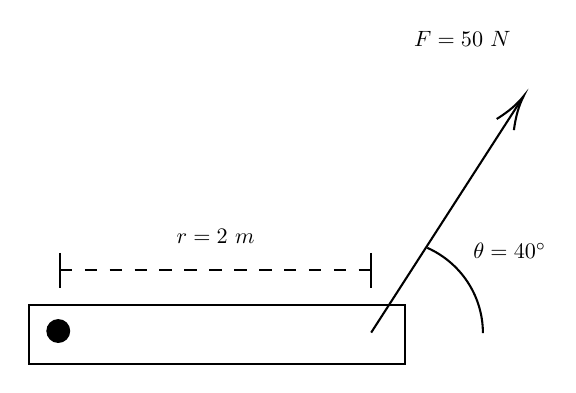
\begin{tikzpicture}[x=0.75pt,y=0.75pt,yscale=-1.5,xscale=1.5]
% Main diagram pieces (from the original)
%Shape: Rectangle
\draw (1,93) -- (122,93) -- (122,112) -- (1,112) -- cycle ;
%Shape: Circle
\draw[fill={rgb,255:red,0;green,0;blue,0},fill opacity=1]
  (7,101.5) .. controls (7,99.57) and (8.57,98) .. (10.5,98)
  .. controls (12.43,98) and (14,99.57) .. (14,101.5)
  .. controls (14,103.43) and (12.43,105) .. (10.5,105)
  .. controls (8.57,105) and (7,103.43) .. (7,101.5) -- cycle ;

%Shape: Arc (angle marker)
\draw[draw opacity=0]
  (129.02,74.78) .. controls (139.52,79.43) and (146.86,89.92) .. (146.89,102.15)
  -- (116.89,102.23) -- cycle ;
\draw
  (129.02,74.78) .. controls (139.52,79.43) and (146.86,89.92) .. (146.89,102.15) ;

%Force arrow
\draw (111,102) -- (158.92,27.68) ;
\draw[shift={(160,26)}, rotate=122.81, line width=0.75]
  (10.93,-3.29) .. controls (6.95,-1.4) and (3.31,-0.3) .. (0,0)
  .. controls (3.31,0.3) and (6.95,1.4) .. (10.93,3.29);

%Dashed radius/lever arm line
\draw[dash pattern={on 4.5pt off 4.5pt}] (11,82) -- (111,82) ;
\draw[shift={(111,82)}, rotate=180, line width=0.75] (0,5.59) -- (0,-5.59);
\draw[shift={(11,82)}, rotate=180,  line width=0.75] (0,5.59) -- (0,-5.59);

% Text nodes
\draw (143,72.4) node [anchor=north west,inner sep=0.75pt,xscale=0.8,yscale=0.8] {$\theta =40^{\circ }$};
\draw (124,4.4)  node [anchor=north west,inner sep=0.75pt,xscale=0.8,yscale=0.8] {$F=50\ \text{N}$};
\draw (61,71)    node [xscale=0.8,yscale=0.8] {$r=2\ \text{m}$};
\end{tikzpicture}
\caption{Main diagram.}
\end{figure}


\textbf{Answer}: Before just plugging in values, let's seperate the force vector into components. The component that pulls perpendicular to the axis is $50 \sin40^\circ$, while $50 \cos40^\circ$ of the force is applied \textit{pulling} the rod against the pivot, which produces no torque. 
% Diagram made with mathcha
\begin{figure}[H]
\centering

\begin{subfigure}{0.48\linewidth}
\centering
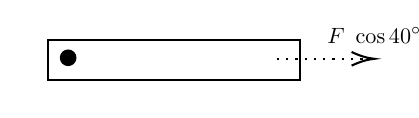
\begin{tikzpicture}[x=0.75pt,y=0.75pt,yscale=-1,xscale=1]
% Tight bounding box around this component
\path[use as bounding box] (200,85) rectangle (375,115);

%Shape: Rectangle
\draw (210,91) -- (331,91) -- (331,110) -- (210,110) -- cycle ;
%Shape: Circle
\draw[fill={rgb,255:red,0;green,0;blue,0},fill opacity=1]
  (216,99.5) .. controls (216,97.57) and (217.57,96) .. (219.5,96)
  .. controls (221.43,96) and (223,97.57) .. (223,99.5)
  .. controls (223,101.43) and (221.43,103) .. (219.5,103)
  .. controls (217.57,103) and (216,101.43) .. (216,99.5) -- cycle ;

%Straight line (cos component)
\draw[dash pattern={on 0.84pt off 2.51pt}] (320,100) -- (365,100) ;
\draw[shift={(367,100)}, rotate=180, color={rgb,255:red,0;green,0;blue,0}, line width=0.75]
  (10.93,-3.29) .. controls (6.95,-1.4) and (3.31,-0.3) .. (0,0)
  .. controls (3.31,0.3) and (6.95,1.4) .. (10.93,3.29);

% Label
\draw (367,93.6) node [anchor=south,inner sep=0.75pt,xscale=0.8,yscale=0.8] {$F\ \cos 40^{\circ }$};
\end{tikzpicture}
\caption{$F\cos\theta$}
\end{subfigure}
\hfill
%------------------------
% (b) Sine component
%------------------------
\begin{subfigure}{0.48\linewidth}
\centering
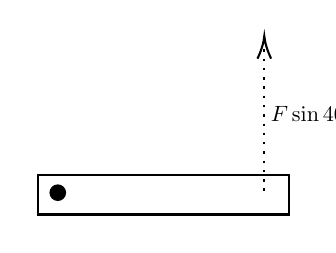
\begin{tikzpicture}[x=0.75pt,y=0.75pt,yscale=-1,xscale=1]
% Tight bounding box around this component
\path[use as bounding box] (405,20) rectangle (540,115);

%Shape: Rectangle
\draw (410,91) -- (531,91) -- (531,110) -- (410,110) -- cycle ;
%Shape: Circle
\draw[fill={rgb,255:red,0;green,0;blue,0},fill opacity=1]
  (416,99.5) .. controls (416,97.57) and (417.57,96) .. (419.5,96)
  .. controls (421.43,96) and (423,97.57) .. (423,99.5)
  .. controls (423,101.43) and (421.43,103) .. (419.5,103)
  .. controls (417.57,103) and (416,101.43) .. (416,99.5) -- cycle ;

%Straight line (sin component)
\draw[dash pattern={on 0.84pt off 2.51pt}] (519,26) -- (519,99) ;
\draw[shift={(519,24)}, rotate=90, color={rgb,255:red,0;green,0;blue,0}, line width=0.75]
  (10.93,-3.29) .. controls (6.95,-1.4) and (3.31,-0.3) .. (0,0)
  .. controls (3.31,0.3) and (6.95,1.4) .. (10.93,3.29);

% Label
\draw (521,61.5) node [anchor=west,inner sep=0.75pt,xscale=0.8,yscale=0.8] {$F\sin 40^{\circ }$};
\end{tikzpicture}
\caption{$F\sin\theta$}
\end{subfigure}

\caption{Components of the applied force.}
\end{figure}

Think back to the wrench example: you don't push or pull a wrench to loosen a bolt; you must apply a force \emph{tangential} or \emph{perpendicular} to the bolt to rotate it. 

Since only the perpendicular component contributes to the torque, we calculate the torque to be $\tau = 50 \sin40^\circ \,\text{N} \,(2 \text{m}) \approx 64.278 \,\text{Newton-meters}$

\begin{Exercise}[title=Door Torque, label=torque1]
A door is connected to a wall by a hinge $0.5 \text{ m}$ from the handle. A person opens the door with a tangential force of $38 \text{ N}$. What is the torque on the door?
\end{Exercise}
\begin{Answer}[ref=torque1]
The torque on the door is equal to $rF\sin\theta$. Since our force is tangential, the sin component is at its max: $\sin 90 = 1$, our torque simplifies to $\tau = rF = 0.5 \cdot 38 = 19 \text{ Newton-Meters}$. 
\end{Answer}
\begin{Exercise}[title=Torque but with a twist!,label=torque2]
A uniform horizontal beam is hinged at the left end and held in place by a force applied at its right end. The beam has length $L=2.0 \text{ m}$. A force of magnitude $F = 20 \text{ N}$ is applied at the right end of the beam, making an angle of $30^\circ$ above the beam.

If the pivot point is at the left end of the beam,
\begin{enumerate}
  \item Find the magnitude of the torque about the hinge.
  \item State whether the torque tends to rotate the beam clockwise or counterclockwise.
\end{enumerate}
\end{Exercise}
\begin{Answer}[ref=torque2]
\begin{enumerate}
  \item Using $\tau = r F \sin\theta$, we can state that the torque is $\tau = (2.0)(10)\sin(30^\circ) = 20(0.5) = 10\ \text{N\cdot m}$.
  \item Because The force has an upward component at the right end, so the beam tends to rotate counterclockwise.
\end{enumerate}
\end{Answer}

\subsection{Torque directions}
\index{torques!applied in opposite directions}
What happens when two torques are applied in \emph{opposite}? Let's take a look at the merry-go-round again, but this time applied with two torques.
% Mathcha
\begin{figure}[H]
\centering
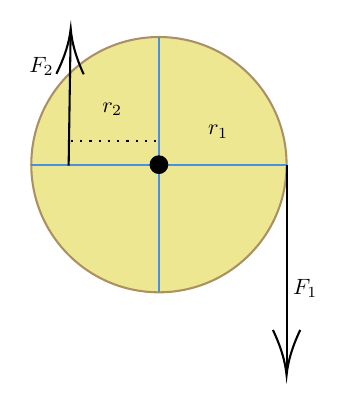
\begin{tikzpicture}[x=0.75pt,y=0.75pt,yscale=-1,xscale=1]

%Shape: Circle
\draw[color={rgb,255:red,170;green,144;blue,99},draw opacity=1,
      fill={rgb,255:red,238;green,231;blue,145},fill opacity=1]
(214,91.5) .. controls (214,57.53) and (241.53,30) .. (275.5,30)
.. controls (309.47,30) and (337,57.53) .. (337,91.5)
.. controls (337,125.47) and (309.47,153) .. (275.5,153)
.. controls (241.53,153) and (214,125.47) .. (214,91.5) -- cycle ;

%Axes/diameter lines (blue)
\draw[color={rgb,255:red,74;green,144;blue,226},draw opacity=1]
(275.5,153) -- (275.5,30) ;
\draw[color={rgb,255:red,74;green,144;blue,226},draw opacity=1]
(214,91.5) -- (337,91.5) ;
%Center point
\draw[fill={rgb,255:red,0;green,0;blue,0},fill opacity=1]
(271.5,91.5) .. controls (271.5,89.29) and (273.29,87.5) .. (275.5,87.5)
.. controls (277.71,87.5) and (279.5,89.29) .. (279.5,91.5)
.. controls (279.5,93.71) and (277.71,95.5) .. (275.5,95.5)
.. controls (273.29,95.5) and (271.5,93.71) .. (271.5,91.5) -- cycle ;


%Force F1 (downward)
\draw (337,91.5) -- (337,191) ;
\draw[shift={(337,193)}, rotate=270, color={rgb,255:red,0;green,0;blue,0}, line width=0.75]
(21.86,-6.58) .. controls (13.9,-2.79) and (6.61,-0.6) .. (0,0)
.. controls (6.61,0.6) and (13.9,2.79) .. (21.86,6.58);

%Force F2 (upward, offset)
\draw (232,92) -- (232.97,28) ;
\draw[shift={(233,26)}, rotate=90.87, color={rgb,255:red,0;green,0;blue,0}, line width=0.75]
(21.86,-6.58) .. controls (13.9,-2.79) and (6.61,-0.6) .. (0,0)
.. controls (6.61,0.6) and (13.9,2.79) .. (21.86,6.58);

%Dashed radius segment and labels
\draw[dash pattern={on 0.84pt off 2.51pt}] (233,80) -- (277,80) ;
\draw (298,71.4) node [anchor=north west,inner sep=0.75pt,xscale=0.8,yscale=0.8] {$r_{1}$};
\draw (247,60.4) node [anchor=north west,inner sep=0.75pt,xscale=0.8,yscale=0.8] {$r_{2}$};

%Force labels
\draw (339,145.65) node [anchor=north west,inner sep=0.75pt,xscale=0.8,yscale=0.8] {$F_{1}$};
\draw (225.91,44.2) node [anchor=east,inner sep=0.75pt,xscale=0.8,yscale=0.8] {$F_{2}$};

\end{tikzpicture}
\caption{Merry-go-round with 2 forces in opposing directions.}
\end{figure}

Torques applied in opposition act \emph{in opposite directions along the axis of rotation}. As torque is a vector defined by the \emph{cross product equation}~\ref{eq:torque_cross}, so its direction is perpendicular to the plane formed by position vector and force which the plane live on. In problems, you will typically see the terms \emph{out of} ($\odot$), or \emph{into} ($\otimes$), the page, corresponding to the $+z$ or $-z$ directions, respectively. Remember these terms by the following visualiations: the out of symbol (\odot) looks like the tip of a feathered dart coming at you, while the into symbol (\otimes) looks like the feathers of a dart. 

To determine which direction a given torque points, one first identifies the sense of rotation the force would produce if acting alone: a force that tends to rotate the object counterclockwise in the plane produces a torque vector pointing out of the page, while a force that tends to rotate the object clockwise produces a torque vector pointing into the page. When two torques are opposite, one must therefore cause clockwise rotation and the other counterclockwise rotation, leading to torque vectors that are equal in line of action but opposite in direction. 

The \emph{net torque}\index{net torque} is the sum of all torques present, similar to how net force is the sum of all forces. Counterclockwise torques are positive, while clockwise torques are negative. Using our merry go round example, we have $F_2$ is \odot while $F_1$ is \otimes.
\begin{align*}
    \tau_{\text{net}} &= \sum \tau \\
    &=+(F_2)(r_2) - (F_1)(r_1)
\end{align*}
Because we know $\tau_1 > \tau_2$, the net torque is going to be negative, characterized with $\otimes$, and clockwise.

\begin{Exercise}[title=Opposing Torques on a Beam, label=opptorque]
A uniform horizontal beam of length $4.0 \text{ m}$ and mass $20 \text{ kg}$ is supported by a pivot located $1.0 \text{ m}$ from the left end. Two forces act on the beam, producing opposing torques about the pivot.
\begin{itemize}
  \item A downward force of $50 \text{ N}$ is applied at the left end of the beam.
  \item A downward force of unknown magnitude $\text{F}$ is applied at the right end of the beam.
  \item The beam is in a state of static equilibrium.
\end{itemize}

Complete the following:
\begin{enumerate}
  \item Find the Weight of the Beam
  \item Write an equation for torque before solving for $F$
  \item Solve for $F$, the unknown force acting on the right end
\end{enumerate}
\end{Exercise}
\begin{Answer}[ref=opptorque]
\begin{enumerate}
  \item Since the beam center is $2.0 \text{ m}$ from the left end, and the pivot is at $1.0 \text{ m}$ from the left end, so the weight is $W= mg = 20(9.8)$,
  $$W = 196\text{ N},\quad \text{acting } 1.0\text{ m right of pivot}$$
  \item We can choose our own torque direction, so let's set counterclockwise be positive. The left end is $1.0\text{ m}$ to the left of the pivot and right end is $3.0\text{ m}$ to the right of the pivot. The beam's weight acts $1.0\text{ m}$ to the right of the pivot.
  
  Since there are no angles and all pivots forces are perpendicular, there are three torques:
  $$\tau_\text{50} = (1.0)(50) = +50 \text{ N} \cdot \text{m}\qquad\text{CCW}$$
  $$\tau_\text{W} = -(1.0)(196) = -196 \text{ N} \cdot \text{m}\qquad\text{CW}$$
  $$\tau_\text{F} = -(3.0)(F) \text{ N} \cdot \text{m}\qquad\text{CW}$$
  So equilibrium is solved by:
  $$50 - 196 - 3F = 0$$
  \item 
  \begin{align*}
    50 - 196 - 3F &= 0 \\
    -146 - 3F &= 0 \\
    -3F &= 146 \\
    F &= -48.7 \text{ N}
  \end{align*}
  The negative informs us that the torques act opposite the direction we assumed, so the force acts $F = 48.7\text{ N upward at the right end}$. 
\end{enumerate}
\end{Answer}

\begin{Exercise}[title=More Complicated Opposing Torque,label=opptorque2]
FIXME assign values to torques, solve 

\tikzset{every picture/.style={line width=0.75pt}} %set default line width to 0.75pt        

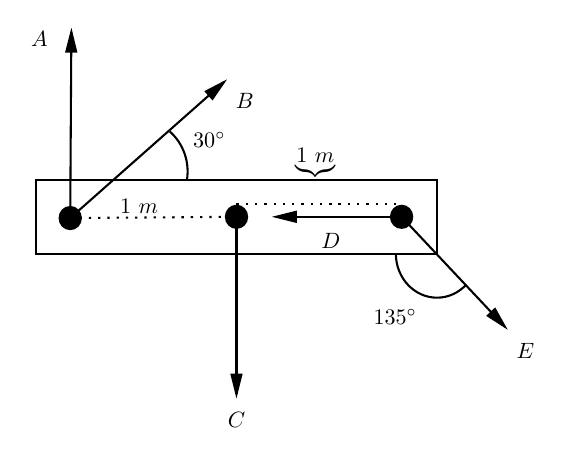
\begin{tikzpicture}[x=0.75pt,y=0.75pt,yscale=-1,xscale=1]
%uncomment if require: \path (0,300); %set diagram left start at 0, and has height of 300

%Shape: Rectangle [id:dp7824893926364507] 
\draw   (4.68,73.89) -- (197.86,73.89) -- (197.86,109.37) -- (4.68,109.37) -- cycle ;
%Shape: Ellipse [id:dp912657781646204] 
\draw  [fill={rgb, 255:red, 0; green, 0; blue, 0 }  ,fill opacity=1 ] (16.05,92.22) .. controls (16.05,89.28) and (18.33,86.9) .. (21.16,86.9) .. controls (23.98,86.9) and (26.27,89.28) .. (26.27,92.22) .. controls (26.27,95.16) and (23.98,97.54) .. (21.16,97.54) .. controls (18.33,97.54) and (16.05,95.16) .. (16.05,92.22) -- cycle ;
%Shape: Ellipse [id:dp9979543530120502] 
\draw  [fill={rgb, 255:red, 0; green, 0; blue, 0 }  ,fill opacity=1 ] (96.16,91.63) .. controls (96.16,88.69) and (98.45,86.31) .. (101.27,86.31) .. controls (104.1,86.31) and (106.39,88.69) .. (106.39,91.63) .. controls (106.39,94.57) and (104.1,96.95) .. (101.27,96.95) .. controls (98.45,96.95) and (96.16,94.57) .. (96.16,91.63) -- cycle ;
%Shape: Ellipse [id:dp5988032294285354] 
\draw  [fill={rgb, 255:red, 0; green, 0; blue, 0 }  ,fill opacity=1 ] (175.7,91.63) .. controls (175.7,88.69) and (177.99,86.31) .. (180.82,86.31) .. controls (183.64,86.31) and (185.93,88.69) .. (185.93,91.63) .. controls (185.93,94.57) and (183.64,96.95) .. (180.82,96.95) .. controls (177.99,96.95) and (175.7,94.57) .. (175.7,91.63) -- cycle ;
%Straight Lines [id:da2304418519139172] 
\draw    (21.16,92.22) -- (21.71,2.55) ;
\draw [shift={(21.73,0.55)}, rotate = 90.36] [fill={rgb, 255:red, 0; green, 0; blue, 0 }  ][line width=0.08]  [draw opacity=0] (12,-3) -- (0,0) -- (12,3) -- cycle    ;
%Straight Lines [id:da19496018549704763] 
\draw    (21.16,92.22) -- (95.23,26.71) ;
\draw [shift={(96.73,25.39)}, rotate = 138.51] [fill={rgb, 255:red, 0; green, 0; blue, 0 }  ][line width=0.08]  [draw opacity=0] (12,-3) -- (0,0) -- (12,3) -- cycle    ;
%Straight Lines [id:da9183149188766027] 
\draw    (101.27,91.63) -- (101.27,177.16) ;
\draw [shift={(101.27,179.16)}, rotate = 270] [fill={rgb, 255:red, 0; green, 0; blue, 0 }  ][line width=0.08]  [draw opacity=0] (12,-3) -- (0,0) -- (12,3) -- cycle    ;
%Straight Lines [id:da6138691044628585] 
\draw    (177.41,91.63) -- (120.32,91.63) ;
\draw [shift={(118.32,91.63)}, rotate = 360] [fill={rgb, 255:red, 0; green, 0; blue, 0 }  ][line width=0.08]  [draw opacity=0] (12,-3) -- (0,0) -- (12,3) -- cycle    ;
%Straight Lines [id:da26125028208728973] 
\draw    (180.82,91.63) -- (230.58,144.58) ;
\draw [shift={(231.95,146.04)}, rotate = 226.78] [fill={rgb, 255:red, 0; green, 0; blue, 0 }  ][line width=0.08]  [draw opacity=0] (12,-3) -- (0,0) -- (12,3) -- cycle    ;
%Shape: Arc [id:dp6523815955840738] 
\draw  [draw opacity=0] (69.13,50.54) .. controls (75.71,56.3) and (78.76,65.24) .. (77.39,73.85) -- (53.58,69.73) -- cycle ; \draw   (69.13,50.54) .. controls (75.71,56.3) and (78.76,65.24) .. (77.39,73.85) ;  
%Shape: Arc [id:dp6151291693574783] 
\draw  [draw opacity=0] (212.01,124.23) .. controls (208.45,128.13) and (203.48,130.55) .. (197.99,130.59) .. controls (187.04,130.65) and (178.12,121.21) .. (178.05,109.49) .. controls (178.05,109.45) and (178.05,109.41) .. (178.05,109.37) -- (197.86,109.37) -- cycle ; \draw   (212.01,124.23) .. controls (208.45,128.13) and (203.48,130.55) .. (197.99,130.59) .. controls (187.04,130.65) and (178.12,121.21) .. (178.05,109.49) .. controls (178.05,109.45) and (178.05,109.41) .. (178.05,109.37) ;  
%Straight Lines [id:da9744888260090975] 
\draw  [dash pattern={on 0.84pt off 2.51pt}]  (21.16,92.22) -- (101.27,91.63) ;
%Straight Lines [id:da43974078659797566] 
\draw  [dash pattern={on 0.84pt off 2.51pt}]  (101.27,85.63) -- (180.82,85.63) ;


% Text Node
\draw (79.18,49.91) node [anchor=north west][inner sep=0.75pt]  [xscale=0.8,yscale=0.8]  {$30^{\circ }$};
% Text Node
\draw (166.09,135.07) node [anchor=north west][inner sep=0.75pt]  [xscale=0.8,yscale=0.8]  {$135^{\circ }$};
% Text Node
\draw (1.16,1.23) node [anchor=north west][inner sep=0.75pt]  [xscale=0.8,yscale=0.8]  {$A$};
% Text Node
\draw (99.82,30.8) node [anchor=north west][inner sep=0.75pt]  [xscale=0.8,yscale=0.8]  {$B$};
% Text Node
\draw (101.27,184.57) node [anchor=north] [inner sep=0.75pt]  [xscale=0.8,yscale=0.8]  {$C$};
% Text Node
\draw (146.73,107.97) node [anchor=south] [inner sep=0.75pt]  [xscale=0.8,yscale=0.8]  {$D$};
% Text Node
\draw (235.05,151.45) node [anchor=north west][inner sep=0.75pt]  [xscale=0.8,yscale=0.8]  {$E$};
% Text Node
\draw (44.02,81.85) node [anchor=north west][inner sep=0.75pt]  [xscale=0.8,yscale=0.8]  {$1\ \text{m}$};
% Text Node
\draw (128.45,57.55) node [anchor=north west][inner sep=0.75pt]  [xscale=0.8,yscale=0.8]  {$\underbrace{1\ \text{m}}$};


\end{tikzpicture}
\end{Exercise}
\begin{Answer}[ref=opptorque2]

\end{Answer}
FIXME exercise of 4 torques without a beam

\section{Moment of Inertia and Rotational $F=ma$}
We know Newton's Second Law by heart now, $F_{net} = ma$. You probably could recite it in your sleep, but what about a rotational equivalent. Recall that from our first circular motion chapter, we have the equation $a = r \alpha$. Let's do some conversions to get this into an angular form:
\begin{align}
    F &= ma \notag \\
    F &= mr\alpha \notag \\
    rF &= mr^2\alpha \notag \\
    \tau &= mr^2\alpha \label{eq:rotNewt2ndLaw}
\end{align}

From Equation~\ref{eq:rotNewt2ndLaw}, we can derive that the ``mass equivalent'' is $mr^2$, since $m$ is multiplied by $a$ in the linear $F=ma$, while $mr^2$ is muliplied by $\alpha$. Thus, we can state that for a point of distance $r$ from the pivot (or axis of rotation), that singular point has \emph{rotation inertia}, also called \emph{moment of inertia}, is defined as $mr^2$. For all point masses on an object, the total inertia is the sum of all point masses of the object.
\begin{mdframed}[frametitle = {Moment of Inertia}, style = important]
    A mass's total moment of inertia is given by the sum of each mass multiplied the distance from the axis of rotation squared.
    \begin{equation}
        I = \sum m r^2\label{eq:momentInertiaSum}
    \end{equation}
    for continuous, solid objects, this becomes
    \begin{equation}
        I = \int r^2 \, dm \label{eq:momentInertiaIntegral}
    \end{equation}
\end{mdframed}
From Equations~\ref{eq:momentInertiaSum} and \ref{eq:momentInertiaIntegral}, we see that mass farther from the axis matters much more than anything closer to the pivot. Or, for two objects, one solid (mass spread evenly throughout) and the other a hollow cylinder or hoop (mass confined to the edges), the hollow cylinder will have a greater moment of inertia.

By finding the net rotational inertia of an object, we can create an equation for the rotational equivalent of Newton's Second Law:
\begin{equation}
    \sum \tau = \tau_{net} = I \alpha
    \label{eq:ialpha}
\end{equation}

\subsection{Relating $\tau = I \alpha$ and other Torque Def'ns}
Since we have already defined angular acceleration, and have just discussed moment of inertia, we can now relate our two torque Equations~\ref{eq:torque_sin} and \ref{eq:ialpha} by equating them, as they both equal net torque.
\begin{equation}
  I \alpha = r F \sin\theta
  \label{eq:torqueequivs}
\end{equation}
This will be useful for solving rotational dynamics problems, and finding any of the variables $I$, $\alpha$, $r$, $F$, or $\theta$ when the others are known.
\begin{Exercise}[title=Angular Acceleration of a Wheel,label=angacc1]
A wheel has \(I=0.80\ \text{kg·m}^2\). A force \(F=25\ \text{N}\) is applied at radius \(r=0.40\ \text{m}\) at an angle \(\theta=60^\circ\) to the radius.

Find \(\alpha\).

\end{Exercise}
\begin{Answer}[ref=angacc1]
Using Equation~\ref{eq:torqueequivs}, we can rearrange to solve for $\alpha$ as $\alpha = \frac{r F \sin\theta}{I}$.
\[
\alpha = \frac{r F \sin\theta}{I} = \frac{0.40 \cdot 25 \sin60}{0.8} \approx 10.825 \text{ rad / s}^2
\]

\end{Answer}

FIXME multiple problems 
FIXME torque and moment of inertua and ang accel eqation 



\section{Parallel-Axis Theorem}

The \textbf{parallel-axis theorem} allows us to calculate the moment of inertia of a rigid body about any axis that is parallel to an axis passing through the center of mass. The theorem states that \index{parallel-axis theorem}
\begin{equation}
I_s = I_{cm} + Md^2
\end{equation}
where $I_s$ is the moment of inertia about the axis of interest, $I_{cm}$ is the moment of inertia about a parallel axis through the center of mass, $M$ is the total mass of the object, and $d$ is the perpendicular distance between the two axes.

In many practical situations, such as a door rotating about its hinges or a rod rotating about one end, the axis of rotation is offset from the center of mass, making direct calculation more difficult. That's where the parallel axis theorem comes in!

\begin{Exercise}[title=Parallel Axis Theorem, label=parallelAxisThm1]
Prove that the Moment of Inertia of the end of a rod is $I_{end} = \frac{1}{3}ML^2$ given that the center of mass of the moment of inertia of a rod is $I_CM = \frac{1}{12}ML^2$.
\end{Exercise}
\begin{Answer}[ref=parallelAxisThm1]
\begin{align*}
  I_{end} &= I_{CM} + MD^2 \\
          &= \frac{1}{2}ML^2 + M\left( \dfrac{L}{2} \right)^2\\
          &= \frac{1}{2}ML^2 + M\left( \dfrac{L^2}{4} \right) \\ 
          &= \left(  \dfrac{1}{12} + \dfrac{1}{4}  \right)ML^2 \\
          &= \left(  \dfrac{4}{12}  \right) ML^2\\
          &= \dfrac{1}{3} ML^2
\end{align*}
\end{Answer}

The parallel-axis theorem shows that the moment of inertia about an offset axis is always greater than the moment of inertia about the center-of-mass axis. The additional term $Md^2$ accounts for the translational motion of the object's center of mass relative to the new axis of rotation. As the distance between the axes increases, the moment of inertia increases accordingly.

If the mass of an object is not evenly distributed, the location of the center of mass shifts, but the parallel-axis theorem remains applicable. Once the center of mass is known, the theorem allows the moment of inertia about any parallel axis to be found by adding the contribution due to the displacement of the center of mass. In this way, the effects of mass distribution are fully captured by the center-of-mass term and the distance between the axes.


\section{Rotational Kinetic Energy and Rolling Motion}
Take a look at this video: \href{https://www.youtube.com/watch?v=CHQOctEvtTY}{Rotational Inertia: The Race Between a Ring and a Disc}.

Let's analyze why the solid cylinder reaches the bottom first.

When two objects roll down an incline without slipping, their acceleration depends not only on gravity, but also on how their mass is distributed. This is because a rolling object must both translate and rotate, so gravitational potential energy is split between translational and rotational kinetic energy. The fraction that goes into rotation depends on the object's moment of inertia.

When an object is rolling, it has both translational kinetic energy and rotational kinetic energy. The total kinetic energy of a rolling object is the sum of these two forms of kinetic energy.

The total rotational kinetic energy of a rolling object comes from all of its individual point masses rotating around the axis. Each point mass has its own rotational kinetic energy $K_i$, and the sum of all these individual kinetic energies gives the total rotational kinetic energy of the object:
\begin{align*}
KE_{\text{rotational}}
&= \sum K_i \\
&= \sum \tfrac{1}{2} m_i r_i^2 \omega^2 \\
&= \tfrac{1}{2} \left( \sum m_i r_i^2 \right) \omega^2 \\
\end{align*}

This gives us the formula for rotational kinetic energy in terms of moment of inertia:
\begin{mdframed}[frametitle = {Rotational Kinetic Energy}, style = important]
The rotational kinetic energy of a rigid body rotating about a fixed axis is given by
\begin{equation}
  KE_{\text{rotational}} = \tfrac{1}{2} I \omega^2
\label{eq:rotKE}
\end{equation}
where $I$ is the moment of inertia of the object about the axis of rotation, and $\omega$ is the angular velocity. This expression applies to rigid bodies rotating about a fixed axis.
\end{mdframed}

Going back to our rolling objects, we can now see that the total kinetic energy of a rolling object is the sum of its translational and rotational kinetic energies:
\begin{mdframed}[frametitle = {Total Kinetic Energy of a Rolling Object}, style = important]
The total kinetic energy of a rolling object is given by
\begin{equation}
  KE_{\text{total}} = KE_{\text{translational}} + KE_{\text{rotational}} = \tfrac{1}{2} mv^2 + \tfrac{1}{2} I \omega^2
\label{eq:totalKErolling}
\end{equation}
where $m$ is the mass of the object, $v$ is its linear velocity, $I$ is its moment of inertia, and $\omega$ is its angular velocity. For rolling without slipping, the translational and rotational motions are linked, but it is still useful to treat their kinetic energies separately.
\end{mdframed}

The moment of inertia $I$ varies depending on how the mass is distributed in the object, and is a measure of how much the object resists rotational motion. For example, a solid disc has a different moment of inertia than a hollow disc of the same mass and radius. This difference in moment of inertia affects how much of the total kinetic energy is rotational versus translational.

The solid disc has most of its mass concentrated closer to the center, resulting in a lower moment of inertia. This means that less of its total kinetic energy is rotational, allowing more energy to be available for translational motion, which leads to a higher linear velocity down the incline.

\begin{mdframed}[frametitle = {Relationship between translational velocity and moment}, style = important]
For rolling objects of the same mass and radius starting from the same height, translational velocity is inversely related to moment of inertia. This relationship can be expressed as:
\begin{equation}
v \propto \frac{1}{I}
\end{equation}
Explicitly, translational velocity is inversely related to moment of inertia. Objects with larger moments of inertia require more energy to rotate, leaving less energy available for translational motion.
\end{mdframed}

Each object has a unique moment of inertia based on its mass distribution, which directly affects its rolling behavior. Here is a reference table with common moments of inertia for various shapes:
\begin{table}[H]
  \centering
  \renewcommand{\arraystretch}{1.5}
  \begin{tabular}{|l|l|}
    \hline
    \textbf{Object and Axis of Rotation} & \textbf{Moment of Inertia} \\
    \hline
    Solid cylinder or disk (symmetry axis) & $I = \tfrac{1}{2}MR^2$ \\
    \hline
    Solid cylinder or disk (central diameter) & $I = \tfrac{1}{4}MR^2 + \tfrac{1}{12}ML^2$ \\
    \hline
    Hoop (symmetry axis) & $I = MR^2$ \\
    \hline
    Hoop (diameter) & $I = \tfrac{1}{2}MR^2$ \\
    \hline
    Solid sphere (about diameter) & $I = \tfrac{2}{5}MR^2$ \\
    \hline
    Thin spherical shell (about diameter) & $I = \tfrac{2}{3}MR^2$ \\
    \hline
    Rod (about center, perpendicular to length) & $I = \tfrac{1}{12}ML^2$ \\
    \hline
    Rod (about one end, perpendicular to length) & $I = \tfrac{1}{3}ML^2$ \\
    \hline
  \end{tabular}
  \caption{Common Moments of Inertia}
  \label{tab:moments_of_inertia}
\end{table}
A visualization of each of these can be found at Georgia State University's HyperPhysics website: \href{http://hyperphysics.phy-astr.gsu.edu/hbase/mi.html#cmi}{HyperPhysics: Moments of Inertia}.

\section{Flywheel Energy Storage, Work, and Angular Momentum}
\index{flywheels}
A flywheel is a rigid body designed to store rotational energy. It typically consists of a heavy wheel or disk mounted on an axle, with much of its mass concentrated away from the axis of rotation. This mass distribution gives the flywheel a large moment of inertia, allowing it to resist changes in rotational speed. There is very little friction in the axle, so once the flywheel is spinning, it can maintain its angular velocity for a long time with minimal energy loss. We often eliminate friction in flywheel friction problems or calculations.

Because of its large moment of inertia, a flywheel can smooth out variations in rotational motion. When energy is added, the flywheel stores it as rotational kinetic energy. When energy is removed, the flywheel releases this stored energy gradually, helping maintain a more uniform angular velocity. For this reason, flywheels are commonly used in engines, generators, and mechanical systems that require steady rotation.

This relies on the principle of \emph{Conservation of Angular Momentum}\index{Conservation of Angular Momentum}, which states that in the absence of \emph{external torques}, the total angular momentum of a system remains constant. For a flywheel, this means that if no external torque acts on it, its angular momentum will not change, allowing it to maintain its rotational speed even when external forces try to slow it down.
\subsection{Angular Momentum}
The connection between angular momentum and torque is direct: torque is the rate at which angular momentum changes. Applying a torque to a flywheel changes its angular momentum by increasing or decreasing its angular velocity. Because of the flywheel's large moment of inertia, a given torque produces only a gradual change in angular speed, contributing to the flywheel's stabilizing effect.
\begin{mdframed}[frametitle = {Angular Momentum and the Conservation of Angular Momentum}, style = important]
The angular momentum \( L \) of a rotating rigid body is given by
\begin{equation}
L = I \omega
\label{eq:angularMomentum1}
\end{equation}
where \( I \) is the moment of inertia of the body about the axis of rotation, and \( \omega \) is its angular velocity. Angular momentum is a \emph{vector} quantity, with both magnitude and direction.

Just as linear momentum can be written as $F=\frac{dp}{dt}$, torque can be expressed as the time rate of change of angular momentum:
\begin{equation}
\tau = \frac{dL}{dt}
\label{eq:derivTorque}
\end{equation}

We can also derive this as a Newtonian cross product between $r$ and $\textbf{p}$, linear momentum. This works because angular momentum is the rotational equivalent of linear momentum, but depends on the choice of origin.
\begin{equation}
L = r \times p
\label{eq:angularMomentum2}
\end{equation}

Just like linear momentum, angular momentum is conserved in a system with no external torques. This is known as the \emph{Conservation of Angular Momentum}:
\begin{equation}
L_{\text{initial}} = L_{\text{final}} \quad (\boldsymbol{\tau}_{\text{net}} = 0)
\end{equation}

\end{mdframed}

This equation shows that torque is responsible for changing angular momentum. Because a flywheel has a large moment of inertia, a given applied torque produces only a small angular acceleration, allowing the flywheel to respond smoothly to changes in applied forces. 

\subsection{Work done by Torque}
Recall that work is a change in energy. Torque also does work when it causes rotation. For a constant torque acting on point mass through an angular displacement $\Delta \theta$ the work done is
\begin{equation}
W = Fr\theta= \tau \Delta \theta
\label{eq:work_rot}
\end{equation}

This comes from the fact that linear work is defined as $W = F \Delta x$, and the arc length of a circle is defined as $s = r \theta$. Thus, we can substitute $r \theta$ for $\Delta x$ in the linear work equation to get the rotational work equation.

\section{Summary}
\begin{table}[H]
\centering
\renewcommand{\arraystretch}{1.5}
\caption{Correspondence Between Linear and Rotational Motion}
\label{tab:linear_rotational_analogy}
\begin{tabular}{|c|c|}
\hline
\textbf{Linear Motion} & \textbf{Rotational Motion} \\
\hline
Position $x$ & Angle $\theta$ \\
\hline
Velocity $v$ & Angular velocity $\omega$ \\
\hline
Acceleration $a$ & Angular acceleration $\alpha$ \\
\hline
Mass $m$ & Moment of inertia $I$ \\
\hline
Force $F$ & Torque $\tau$ \\
\hline
Momentum $p = mv$ & Angular momentum $L = I\omega$ \\
\hline
$F = \dfrac{dp}{dt}$ & $\tau = \dfrac{dL}{dt}$ \\
\hline
Work $W = F \Delta x$ & Work $W = \tau \Delta \theta$ \\
\hline
Kinetic Energy $\tfrac{1}{2}mv^2$ & Rotational KE $\tfrac{1}{2}I\omega^2$ \\
\hline
Power $P = Fv$ & Power $P = \tau \omega$ \\
\hline
\end{tabular}
\end{table}
